\documentclass[11pt]{article}

\usepackage[margin=1in]{geometry}
\usepackage[T1]{fontenc}
\usepackage[utf8]{inputenc}
\usepackage{lmodern}
\usepackage{booktabs}
\usepackage{graphicx}
\usepackage{hyperref}
\usepackage{enumitem}
\usepackage{amsmath}

\title{Technical Memo: Direct Vocabulary Steering in Larger Dual-Stream Models}
\author{GPT-OSS Interpretability Project}
\date{March 11, 2026}

\begin{document}
\maketitle

\begin{abstract}
This memo summarizes a first larger-scale evaluation of direct vocabulary
steering in locally trained dual-stream and CASCADE-family language models.
The intervention is simple: for a binary contrast with first divergent answer
tokens $\text{token}_A$ and $\text{token}_B$, inject the exact vocabulary
direction
\[
\Delta v = W[\text{token}_A] - W[\text{token}_B]
\]
into the contextual stream and measure the resulting change in local answer
preference. We evaluate five GPT-2-vocabulary models ranging from a matched
71M-parameter single-stream/CASCADE pair to larger 12-layer CASCADE+PLS
variants. The core result is positive: the effect is sign-consistent, local
under the current decomposition, and reasonably disciplined with respect to
off-target drift across all evaluated models. The strongest scientific
comparison is the matched 71M pair, where CASCADE is slightly stronger than the
single-stream baseline on two of three tasks, but not by a large enough margin
to justify a strong architecture-superiority claim. The current bottleneck is
not runtime but panel quality: one capitalization case remains tokenizer-dirty
and should be replaced before this result is treated as a clean steering
benchmark.
\end{abstract}

\section{Memo Context}

This document is a technical memo in the style of a compact steering paper. It
is not intended as a full conference submission. The aim is to record the
question, design, current evidence, and next experimental decisions in a form
that is easy to cite internally and easy to extend into a later paper.

\paragraph{Implementation status.}
The repo now has a scaffolded package split between
\texttt{gpt\_oss\_interp/steering/},
\texttt{gpt\_oss\_interp/distillation/}, and
\texttt{gpt\_oss\_interp/common/}. This matters for the next phase of work:
per-channel probing, readout decomposition, and symbolic-slice interventions
should now be implemented natively under \texttt{steering/}, while
teacher-student and CASCADE-target code should live under
\texttt{distillation/}. The split is still a scaffold, not a completed code
migration, but it establishes the intended structure for future work.

\paragraph{Model aliases.}
To keep the tables compact, we use short aliases:
\begin{itemize}[leftmargin=1.5em]
\item \textbf{SS-71}: matched 71M single-stream GPT-2-vocab model
\item \textbf{C-71}: matched 71M CASCADE GPT-2-vocab model
\item \textbf{CP-71}: 71M CASCADE+PLS GPT-2-vocab model
\item \textbf{CP-80}: larger CASCADE+PLS Codelion-80M model
\item \textbf{CP-124}: larger CASCADE+PLS GPT-2-base-scale model
\end{itemize}

\section{Introduction}

Standard activation steering work usually applies directions in residual space
or hidden-state space, where token identity, context, syntax, and latent task
variables are entangled. The motivating idea behind the present line of work is
that dual-stream or symbolic-transformer-style architectures may support a more
direct and more interpretable intervention. If vocabulary geometry remains
legible inside the model, then a human-readable token contrast should function
as a usable steering direction rather than merely as a diagnostic object.

The concrete claim examined here is narrower than a general claim about model
control. We ask whether the exact vocabulary contrast between two answer tokens
can be injected into the contextual stream and produce a predictable local
change in answer preference. We also ask whether this remains true in larger
models, and whether CASCADE appears cleaner than a matched single-stream
baseline.

\section{Related Framing}

This memo sits at the intersection of three lines of prior internal work.

\paragraph{Causal specialization and controllability.}
Earlier capitalization-ablation work argued that per-layer supervision (PLS)
creates heads with larger and more localized causal effects, summarized under
the ``hydra effect'' framing: standard models route around local damage,
whereas more modular models do not. The current steering experiment tests a
closely related but distinct question: whether a clean intervention direction
exists, not merely whether ablation damage is localized.

\paragraph{Bregman geometry and steerability.}
The Bregman-geometry notebooks proposed that PLS and CASCADE may improve the
conditioning of the output geometry and therefore make steering easier or more
disciplined. The present experiment does not directly estimate Hessian
conditioning. Instead, it asks whether the resulting intervention behavior
already looks local and low-crosstalk in practice.

\paragraph{Architecture-specific interpretability.}
The broader thesis behind symbolic and dual-stream models is that if a token
space remains structurally meaningful inside the model, then direct
vocabulary-based interventions should become more plausible than they are in a
standard residual-stream architecture.

\section{Experimental Question}

We evaluate the following question:

\begin{quote}
Can a larger dual-stream or CASCADE-family model be steered by injecting an
exact vocabulary-space contrast into the contextual stream, and does this yield
sign-consistent, local, and reasonably selective behavioral change?
\end{quote}

This decomposes into four operational tests:

\begin{enumerate}[leftmargin=1.5em]
\item \textbf{Sign correctness:} positive and negative scales move the local
answer preference in opposite predicted directions.
\item \textbf{Locality:} the effect appears at the first divergent token rather
than being mediated primarily by suffix or tail behavior.
\item \textbf{Collateral discipline:} off-target effects remain smaller than
the on-target effect.
\item \textbf{Architecture sensitivity:} a matched CASCADE model may show a
cleaner response than a matched single-stream baseline.
\end{enumerate}

\section{Methods}

\subsection{Intervention}

For a case with binary choices $A$ and $B$, let $\text{token}_A$ and
$\text{token}_B$ denote the first divergent completion tokens under the active
tokenizer. Let $W$ denote the model's tied embedding/unembedding matrix. The
steering direction is
\[
\Delta v = W[\text{token}_A] - W[\text{token}_B].
\]

For scale $\alpha$, we inject $\alpha \Delta v$ into the contextual stream
$x_e$ after a selected transformer block. This is a direct vocabulary
intervention rather than a learned steering vector.

\paragraph{Scope note.}
All experiments in this memo use $\Delta v$ as one whole $d_{\mathrm{model}}$
vector. We do \emph{not} yet exploit a stronger dual-stream-specific
intervention family in which the symbolic stream $x_t$ is channelized by head
and token embeddings can be written per head or composed across heads. That
intervention family is unavailable in a standard transformer and remains an
important next step. The correct way to open that space is not by arbitrary
head mixing. It requires ACL-style differential probing first: identify which
channels behave like entity trackers, recency channels, answer selectors, or
generic amplifiers, then intervene on one channel at a time before attempting
mixed-token channel composites.

\paragraph{Implementation note.}
The intended home for that next-phase work is now
\texttt{gpt\_oss\_interp/steering/}: probing in
\texttt{steering/probing.py}, causal symbolic-slice interventions in
\texttt{steering/interventions.py}, null baselines in
\texttt{steering/controls.py}, and readout decomposition in
\texttt{steering/readouts.py}. Shared artifact schemas should remain in
\texttt{gpt\_oss\_interp/common/artifacts.py}.

\subsection{Evaluation Panel}

The same three-case panel was used in all runs:
\begin{itemize}[leftmargin=1.5em]
\item \texttt{caps\_005}
\item \texttt{induction\_009}
\item \texttt{coref\_010}
\end{itemize}

All large-model runs used raw GPT-2 tokenization. This fixed the pathological
reduced-vocabulary collapse seen in the earlier small-model run, especially for
\texttt{coref\_010}. One capitalization issue remains: \texttt{caps\_005}
still diverges at \texttt{" d"} vs.\ \texttt{" Dakota"} rather than at a clean
full-token capitalization contrast.

\subsection{Models}

We evaluated five GPT-2-vocabulary checkpoints:

\begin{center}
\begin{tabular}{lccc}
\toprule
Alias & Stream mode & Scale class & Notes \\
\midrule
\textbf{SS-71} & single-stream & 71M class & matched baseline \\
\textbf{C-71} & CASCADE & 71M class & matched CASCADE pair \\
\textbf{CP-71} & CASCADE + PLS & 71M class & same-scale variant \\
\textbf{CP-80} & CASCADE + PLS & 80M+ class & 12-layer model \\
\textbf{CP-124} & CASCADE + PLS & GPT-2-base class & 12-layer model \\
\bottomrule
\end{tabular}
\end{center}

The matched pair of greatest interest is:
\begin{itemize}[leftmargin=1.5em]
\item \textbf{SS-71}
\item \textbf{C-71}
\end{itemize}

\subsection{Sweep}

\begin{itemize}[leftmargin=1.5em]
\item Layers: 0--5
\item Scales: $\{-2,-1,-0.5,0.5,1,2\}$
\item Target and off-target evaluation: every source-case direction was tested
against all three target cases
\end{itemize}

\subsection{Metrics}

\paragraph{Local gap shift.}
At the first divergent answer token, we measure
\[
\Delta_{\mathrm{local}} =
\left(\mathrm{logit}_A - \mathrm{logit}_B\right)_{\mathrm{intervened}} -
\left(\mathrm{logit}_A - \mathrm{logit}_B\right)_{\mathrm{baseline}}.
\]

\paragraph{Total gap shift.}
For the full answer choices,
\[
\Delta_{\mathrm{total}} =
\left(\mathrm{score}(A) - \mathrm{score}(B)\right)_{\mathrm{intervened}} -
\left(\mathrm{score}(A) - \mathrm{score}(B)\right)_{\mathrm{baseline}}.
\]

\paragraph{Tail fraction.}
Tail fraction summarizes how much of the total shift is not explained by the
local answer-token shift under the current decomposition.

\paragraph{Off-target drift.}
For a source-case direction, we compute the same local shift on the other two
cases and compare that drift to the strongest on-target shift.

\section{Results}

\subsection{Baseline behavior}

All five large models were baseline-correct on all three panel cases. This is
already an improvement over the reduced-vocabulary small-model run, where one
coreference case failed at baseline due to tokenization collapse.

\begin{figure}[t]
\centering
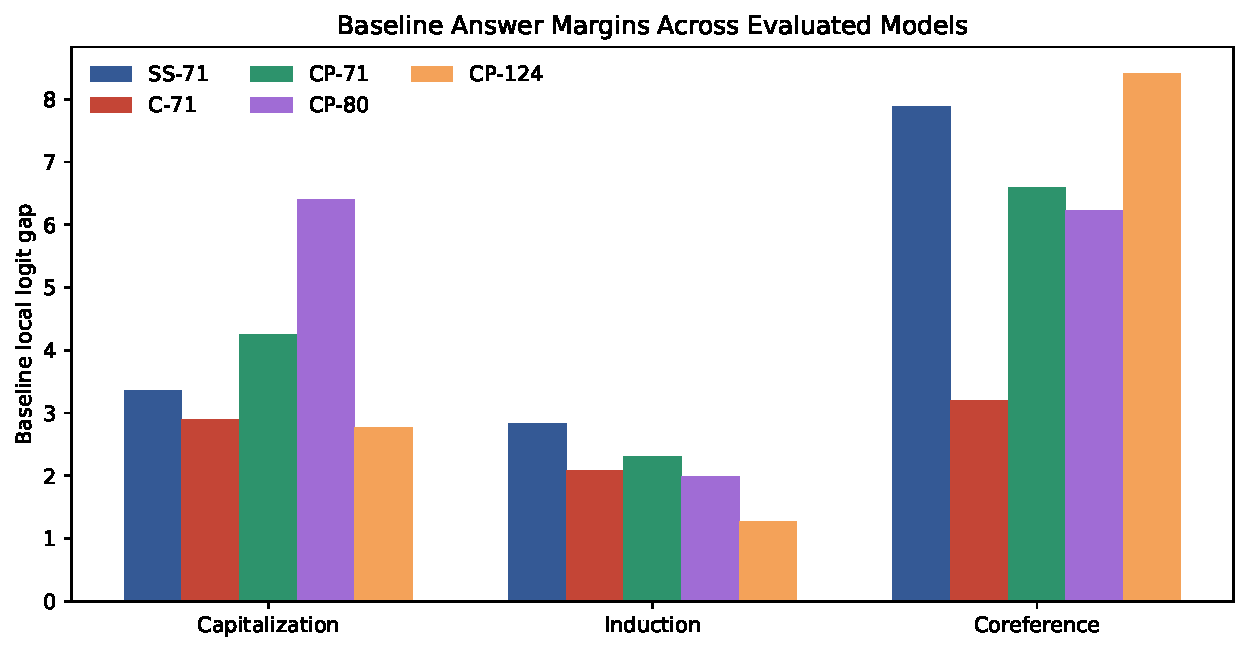
\includegraphics[width=0.88\textwidth]{figs/fig_baseline_local_gaps.pdf}
\caption{Baseline local answer margins for all evaluated models. All five large
models are baseline-correct on the three-case panel before steering is applied.}
\label{fig:baseline-gaps}
\end{figure}

\subsection{Main steering result}

Across all five models and all three cases:

\begin{itemize}[leftmargin=1.5em]
\item sign correctness was perfect in the tested sweep;
\item locality was effectively perfect under the current metric;
\item the direct vocabulary intervention remained bidirectional and causal.
\end{itemize}

This supports the narrow claim that direct vocabulary steering is not merely a
small-model artifact.

\begin{figure}[t]
\centering
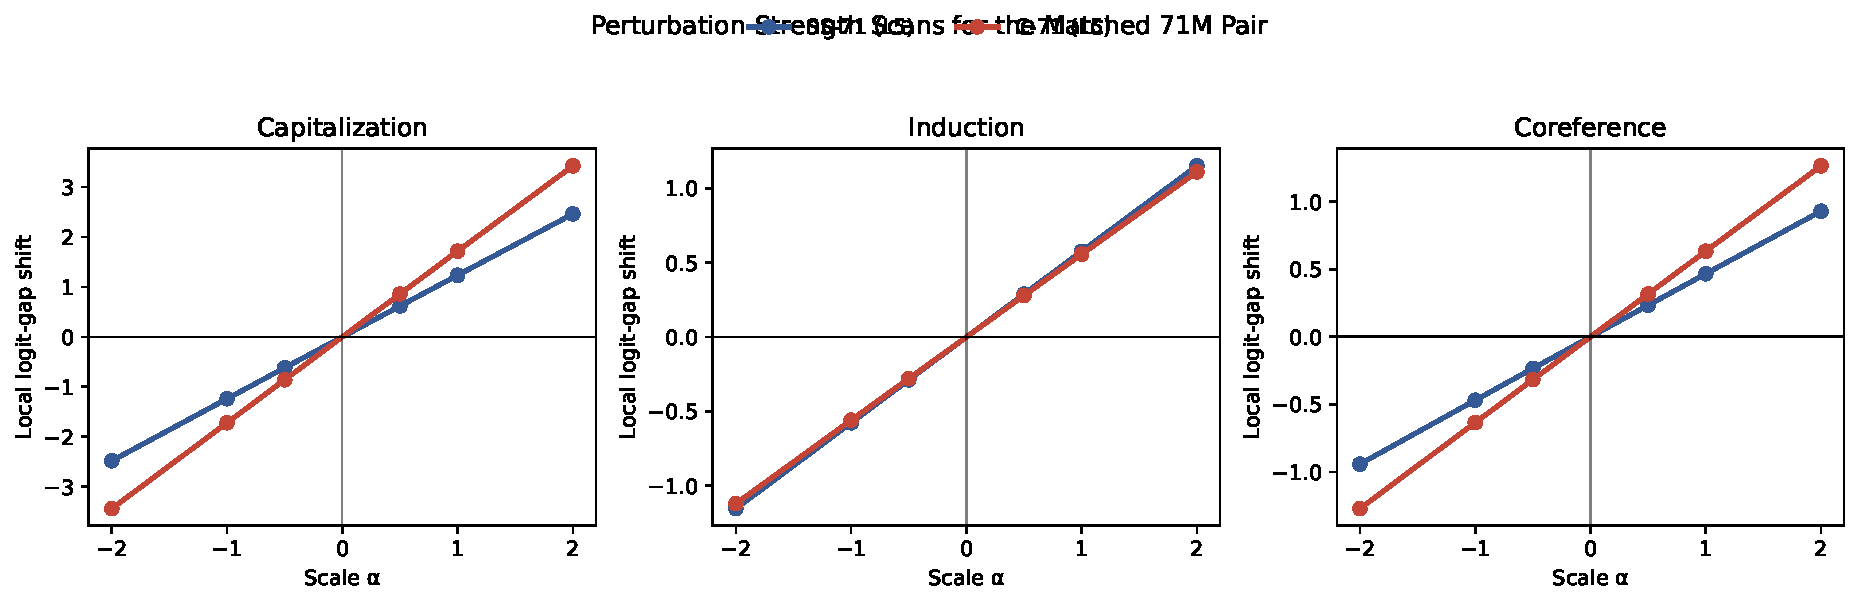
\includegraphics[width=\textwidth]{figs/fig_matched_pair_strength_scans.pdf}
\caption{Perturbation-strength scans for the matched 71M pair. The curves show
sign-consistent, bidirectional local steering across all three cases.}
\label{fig:strength-scans}
\end{figure}

\subsection{Matched 71M comparison}

The most informative comparison is the matched 71M pair:

\begin{itemize}[leftmargin=1.5em]
\item \textbf{SS-71} (single-stream)
\item \textbf{C-71} (CASCADE)
\end{itemize}

Best absolute on-target local shifts:

\begin{center}
\begin{tabular}{lccc}
\toprule
Model & \texttt{caps\_005} & \texttt{induction\_009} & \texttt{coref\_010} \\
\midrule
single-stream 71M & 2.48 & 1.15 & 0.94 \\
CASCADE 71M & 3.44 & 1.12 & 1.27 \\
\bottomrule
\end{tabular}
\end{center}

Interpretation:
\begin{itemize}[leftmargin=1.5em]
\item CASCADE is slightly stronger on capitalization and coreference.
\item Induction is essentially tied.
\item The result favors CASCADE, but not strongly enough to support a large
architecture-superiority claim.
\end{itemize}

\begin{figure}[t]
\centering
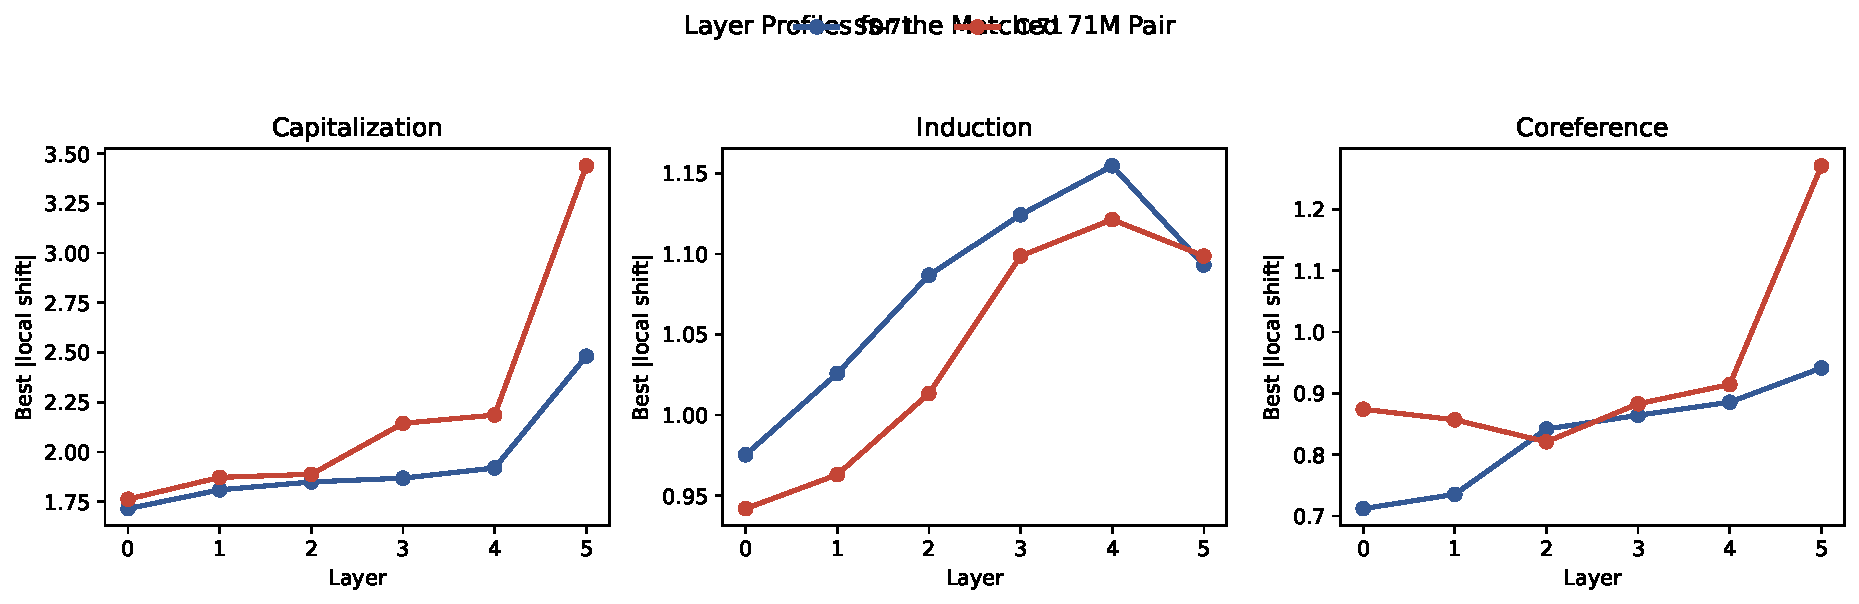
\includegraphics[width=\textwidth]{figs/fig_matched_pair_layer_profiles.pdf}
\caption{Best absolute local steering effect by layer for the matched 71M pair.
The largest effects occur in later layers, with CASCADE modestly stronger on
two of the three cases.}
\label{fig:layer-profiles}
\end{figure}

\subsection{Off-target drift}

For the matched 71M pair, mean off-target drift is small relative to the
strongest on-target effect:

\begin{center}
\begin{tabular}{lccc}
\toprule
Model & Source case & Best on-target & Mean off-target / best on-target \\
\midrule
single-stream 71M & \texttt{caps\_005} & 2.48 & 0.033 \\
single-stream 71M & \texttt{induction\_009} & 1.15 & 0.026 \\
single-stream 71M & \texttt{coref\_010} & 0.94 & 0.072 \\
CASCADE 71M & \texttt{caps\_005} & 3.44 & 0.022 \\
CASCADE 71M & \texttt{induction\_009} & 1.12 & 0.072 \\
CASCADE 71M & \texttt{coref\_010} & 1.27 & 0.098 \\
\bottomrule
\end{tabular}
\end{center}

This is good enough to say that the learned effect is not simply a global blunt
perturbation.

\begin{figure}[t]
\centering
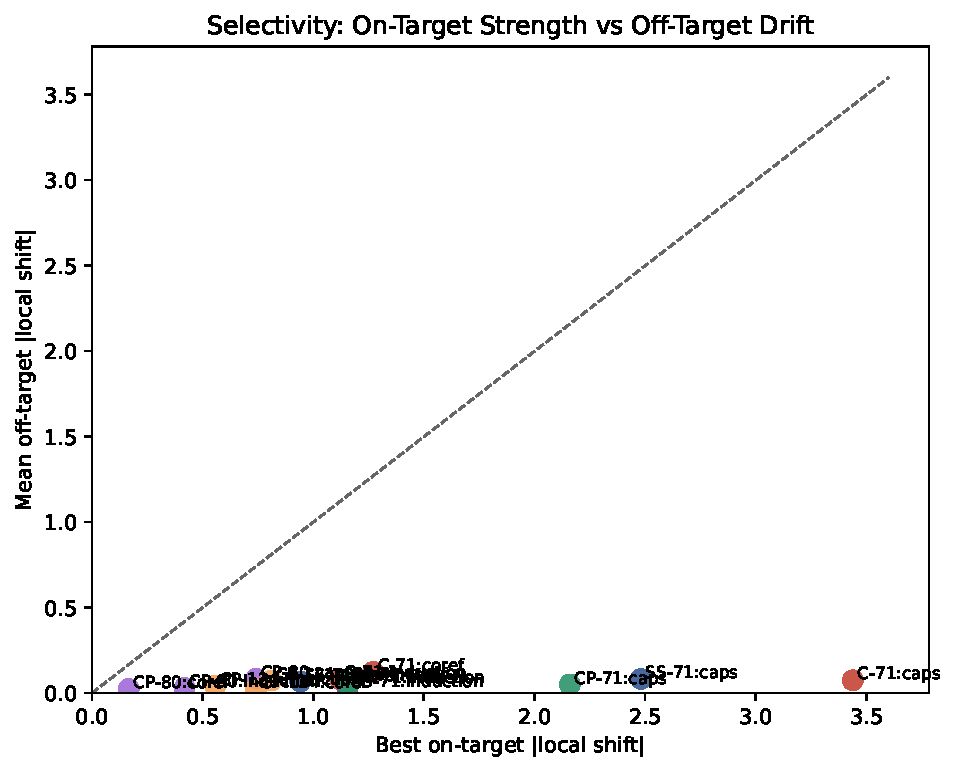
\includegraphics[width=0.78\textwidth]{figs/fig_selectivity_scatter.pdf}
\caption{Selectivity summary across all evaluated models. Each point compares
the strongest on-target effect for a source case with the mean off-target drift
caused by that same direction. Points well below the diagonal indicate
reasonably disciplined steering.}
\label{fig:selectivity}
\end{figure}

\subsection{Larger 12-layer CASCADE models}

The larger CASCADE+PLS models remained baseline-correct but showed smaller
steering magnitudes at the tested scales than the 71M pair. This likely reflects
intervention mismatch rather than disappearance of the effect. Plausible reasons
include:

\begin{itemize}[leftmargin=1.5em]
\item the layer subset 0--5 no longer targets the most responsive depth range;
\item the same scales are too conservative for larger representations;
\item the chosen contextual injection site may be suboptimal for the 12-layer
models.
\end{itemize}

\section{Discussion}

The most important point is that the direct-vocabulary effect survives contact
with larger models. This is the main empirical advance over the earlier small
checkpoint work.

The second point is methodological. Once the experiment is moved to raw GPT-2
tokenization and to stronger checkpoints, the intervention becomes much cleaner
and off-target drift becomes substantially smaller. This means that the current
bottleneck is no longer hardware or even model quality; it is benchmark panel
quality.

The third point is architectural. The matched 71M pair suggests that CASCADE is
at least competitive and perhaps modestly cleaner than the single-stream model
for direct vocabulary steering. However, the gap is not large. At this stage the
best-supported claim is:

\begin{quote}
Direct vocabulary steering works in both matched single-stream and CASCADE
models, with a slight advantage for CASCADE on some tasks.
\end{quote}

\begin{figure}[t]
\centering
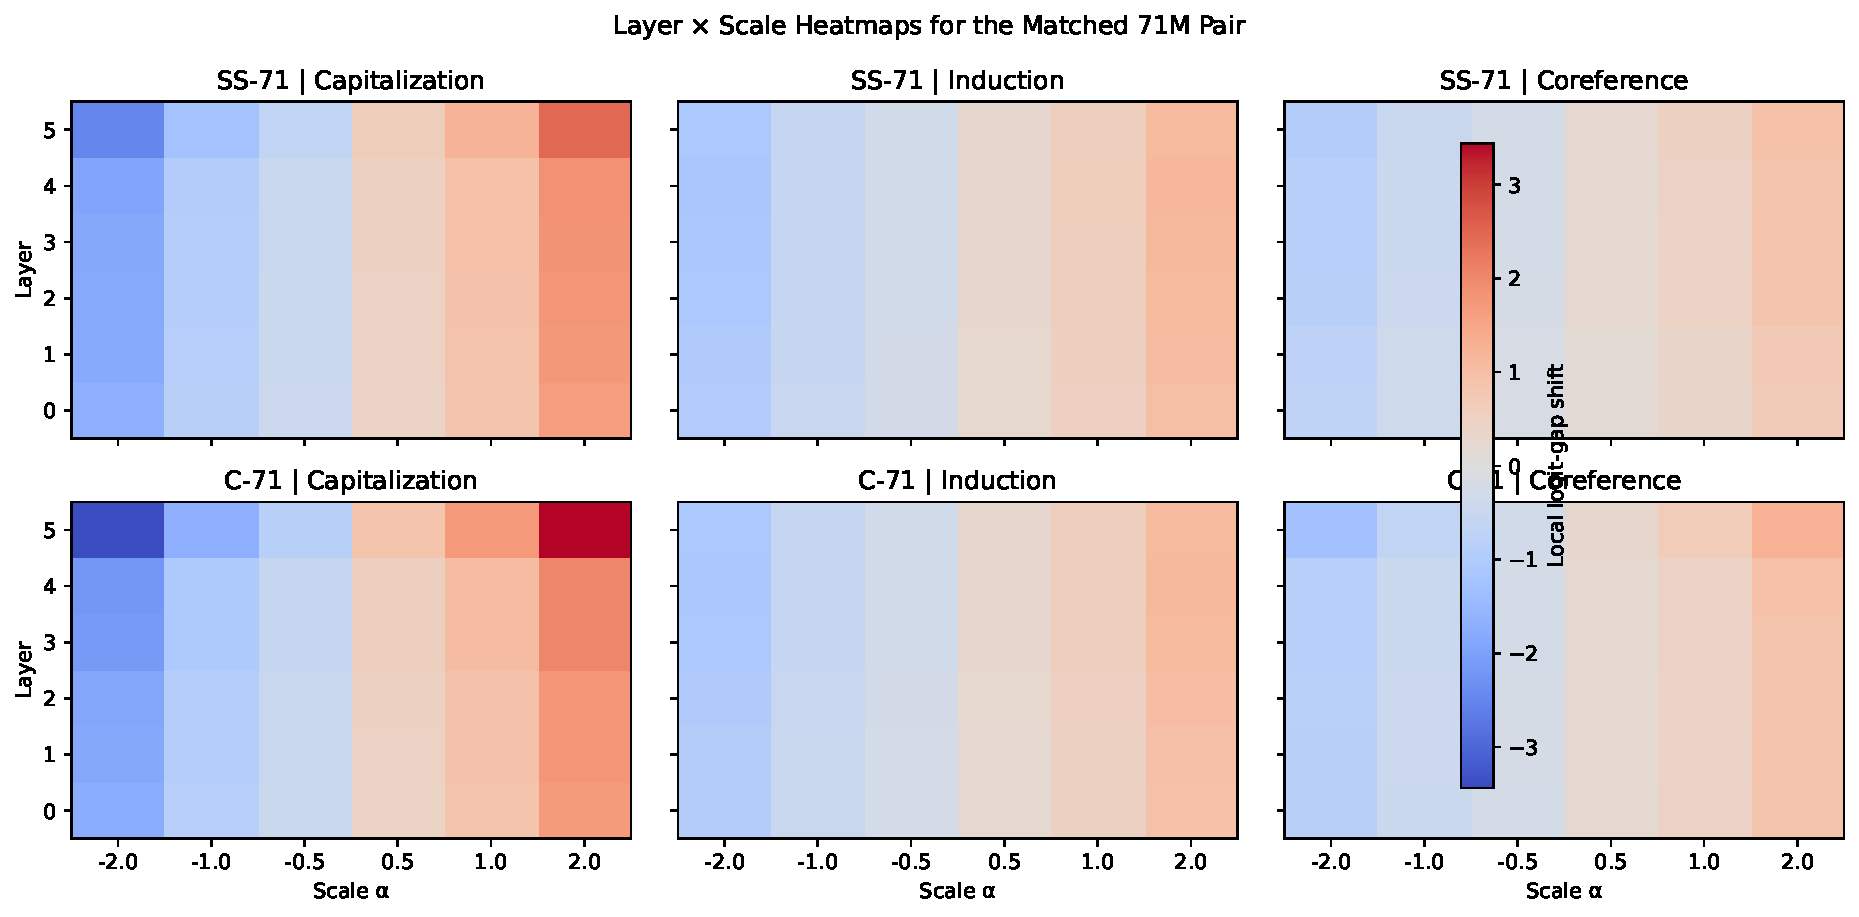
\includegraphics[width=\textwidth]{figs/fig_matched_pair_heatmaps.pdf}
\caption{Layer $\times$ scale heatmaps for the matched 71M pair. These panels
summarize sign symmetry, layer preference, and relative effect magnitude in a
single view.}
\label{fig:heatmaps}
\end{figure}

\section{Limitations}

\begin{enumerate}[leftmargin=1.5em]
\item \textbf{Tokenizer cleanliness is not fully solved.}
\texttt{caps\_005} remains a dirty capitalization case and should not anchor a
publication-quality benchmark.

\item \textbf{The panel is too small.}
Three cases are enough for feasibility, not enough for a robust claim about the
generality of the effect.

\item \textbf{Layer specificity is still weak.}
The strongest effects remain concentrated in late layers for the 71M pair
rather than in a sharply localized intervention band.

\item \textbf{The larger 12-layer models need retuning.}
The current sweep was held fixed to preserve comparability, not to optimize each
model family.
\end{enumerate}

\section{Conclusion}

The present evidence supports a positive but narrow conclusion: exact
vocabulary-space contrasts can be used as causal steering directions in larger
dual-stream and CASCADE-family models, and this effect remains local and
reasonably selective under the current evaluation. The best current evidence
comes from the matched 71M GPT-2-vocabulary pair, where CASCADE is slightly
stronger than the single-stream baseline but not decisively so.

The immediate next step is straightforward. Replace the dirty capitalization
case with a tokenizer-clean contrast, expand the panel modestly, and rerun the
matched 71M comparison. That is the shortest path to a memo that could support a
cleaner literature-style steering claim.

\section{Artifacts}

Primary artifact directory:
\begin{itemize}[leftmargin=1.5em]
\item \texttt{runs/direct\_vocab\_large\_models\_cpu/}
\end{itemize}

Key files:
\begin{itemize}[leftmargin=1.5em]
\item \texttt{runs/direct\_vocab\_large\_models\_cpu/direct\_vocab\_steering.json}
\item \texttt{runs/direct\_vocab\_large\_models\_cpu/report.md}
\item \texttt{scripts/run\_direct\_vocab\_steering.py}
\end{itemize}

\end{document}
